\documentclass[runningheads,a4paper]{llncs}

\usepackage[american]{babel}

\usepackage{graphicx}

%extended enumerate, such as \begin{compactenum}
\usepackage{paralist}

%put figures inside a text
%\usepackage{picins}
%use
%\piccaptioninside
%\piccaption{...}
%\parpic[r]{\includegraphics ...}
%Text...

%Sorts the citations in the brackets
%\usepackage{cite}

%for easy quotations: \enquote{text}
\usepackage{csquotes}

\usepackage[T1]{fontenc}

%enable margin kerning
\usepackage{microtype}

%better font, similar to the default springer font
\usepackage[%
rm={oldstyle=false,proportional=true},%
sf={oldstyle=false,proportional=true},%
tt={oldstyle=false,proportional=true,variable=true},%
qt=false%
]{cfr-lm}
%
%if more space is needed, exchange cfr-lm by mathptmx
%\usepackage{mathptmx}

%for demonstration purposes only
\usepackage[math]{blindtext}

\usepackage[
%pdfauthor={},
%pdfsubject={},
%pdftitle={},
%pdfkeywords={},
bookmarks=false,
breaklinks=true,
colorlinks=true,
linkcolor=black,
citecolor=black,
urlcolor=black,
%pdfstartpage=19,
pdfpagelayout=SinglePage
]{hyperref}
%enables correct jumping to figures when referencing
\usepackage[all]{hypcap}

\usepackage[capitalise,nameinlink]{cleveref}
%Nice formats for \cref
\crefname{section}{Sect.}{Sect.}
\Crefname{section}{Section}{Sections}
\crefname{figure}{Fig.}{Fig.}
\Crefname{figure}{Figure}{Figures}

\usepackage{xspace}
%\newcommand{\eg}{e.\,g.\xspace}
%\newcommand{\ie}{i.\,e.\xspace}
\newcommand{\eg}{e.\,g.,\ }
\newcommand{\ie}{i.\,e.,\ }

%introduce \powerset - hint by http://matheplanet.com/matheplanet/nuke/html/viewtopic.php?topic=136492&post_id=997377
\DeclareFontFamily{U}{MnSymbolC}{}
\DeclareSymbolFont{MnSyC}{U}{MnSymbolC}{m}{n}
\DeclareFontShape{U}{MnSymbolC}{m}{n}{
    <-6>  MnSymbolC5
   <6-7>  MnSymbolC6
   <7-8>  MnSymbolC7
   <8-9>  MnSymbolC8
   <9-10> MnSymbolC9
  <10-12> MnSymbolC10
  <12->   MnSymbolC12%
}{}
\DeclareMathSymbol{\powerset}{\mathord}{MnSyC}{180}

% correct bad hyphenation here
\hyphenation{op-tical net-works semi-conduc-tor}
 
\begin{document}

%Works on MiKTeX only
%hint by http://goemonx.blogspot.de/2012/01/pdflatex-ligaturen-und-copynpaste.html
%also http://tex.stackexchange.com/questions/4397/make-ligatures-in-linux-libertine-copyable-and-searchable
%This allows a copy'n'paste of the text from the paper
\input glyphtounicode.tex
\pdfgentounicode=1

\title{Recommendation Generation for Performance Improvement by using Cross-Organizational Process Mining}
%If Title is too long, use \titlerunning
\titlerunning{Cross-Organizational Process Mining}

%Single insitute
\author{Onur Y{\i}lmaz \and P{\i}nar Karag\"{o}z}
%If there are too many authors, use \authorrunning
%\authorrunning{First Author et al.}
\institute{Computer Engineering Department, Middle East Technical University, Turkey}
%\email{yilmaz.onur@metu.edu.tr} 
%\email{karagoz@ceng.metu.edu.tr}
%Multiple insitutes
%Currently disabled
%
\iffalse
%Multiple institutes are typeset as follows:
\author{Firstname Lastname\inst{1} \and Firstname Lastname\inst{2} }
%If there are too many authors, use \authorrunning
%\authorrunning{First Author et al.}

\institute{
Insitute 1\\
\email{...}\and
Insitute 2\\
\email{...}
}
\fi
			
\maketitle

\begin{abstract}
Process mining is a relatively young and developing research area with the main idea of discovering, monitoring and improving processes by extracting information from the event logs. With the increase of cloud computing and shared infrastructures, event logs of multiple organizations are available for analysis where cross-organizational process mining stands with the opportunity for organizations learning from each other. The approach proposed in this study mines process models of organizations and calculates performance indicators; followed by clustering of organizations based on performance indicators and finally spots mismatches between the process models to generate recommendations. This approach is implemented as extensible and configurable plugin set in ProM framework and tested by synthetic and real life logs where successful and suitable results are achieved within evaluation metrics. Generated recommendation results indicate that the use of this approach considerably helps users to focus on the areas of process models with potential performance improvement, which are difficult to spot manually and visually.
\end{abstract}

\keywords{Process Mining, Cross-organizational Process Mining, Recommendation Generation, Process Performance Improvement}


\section{Introduction}
\label{sec:introduction}

Process mining is a relatively young and developing research area with the roots in computational intelligence, data mining; and process modeling and analysis \cite{van2012process}. Main idea in this research area is to discover, monitor and improve processes by extracting information from event logs. Traditional process mining approaches work on a single organization; however, with the increase of cloud computing and shared infrastructures, event logs of multiple organizations are currently available for analysis where cross-organizational process mining stands out. In cross-organizational process mining area, recent studies focus on commonality and collaboration between organizations. Studies focus on how similar the process models and behaviors of organizations under cross comparison \cite{buijs2012towards} and challenges based on partitioning of tasks and process models between organizations \cite{van2011intra}. This study is based on the environment where processes are executed on several organizations and cross-organizational process mining is applied with the idea of unsupervised learning where predictor variables related to performances of organizations are used.

The approach proposed in this thesis is a four-stage solution and it starts with mining the process models of organizations; followed by performance indicator analysis and then mismatch pattern analysis. Finally recommendation generation stage is undertaken to create learning opportunities for each organization. With this approach it is aimed to help business process management users to focus on the potentially important parts of their business maps. Proposed methodology is implemented in ProM framework \cite{verbeek2010prom} as a set of plugins corresponding for each stage and packaged under the name of \textit{CrossOrgProcMin} and tested on a synthetic and real-life event logs. Performance of methodology is assessed with a defined evaluation metrics for each stage and resulting recommendations are presented to show how this approach helps users to focus on learning opportunities between organizations with a performance improvement potential.

The rest of the paper is organized as follows:
\begin{itemize}
	\item In Chapter~\ref{sec:relatedwork}, related studies in process mining area are presented. 
	\item In Chapter~\ref{sec:background}, background information for the relevant topics is explained.
	\item In Chapter~\ref{sec:methodology}, methodology proposed in this study is presented with detail.
	\item In Chapter~\ref{sec:results-and-discussions}, methodology of this study is applied on datasets and results are discussed.
	\item In Chapter~\ref{sec:conclusion-and-future-work}, summary of this study is presented with the final remarks and pointers for future work. 
\end{itemize}
\section{Related Work}
\label{sec:relatedwork}

In this section, studies related to the work presented in this thesis are summarized. Firstly, studies in the process mining area are explained and then studies from cross-organizational process mining, which is the main topic of this research, is introduced. Following these, studies related to similarity in process mining is mentioned. Finally, performance and conformance analysis approaches in process mining area are presented.

 Within the process mining framework, there are various different process mining algorithms proposed which have the same aim of discovering underlying processes. Considering the underlying approaches undertaken, algorithms can be grouped as $\alpha$-algorithms \cite{van2004workflow, de2004process}, inductive approaches \cite{herbst1998integrating, herbst2000dealing}, hierarchical clustering \cite{greco2005mining}, genetic approaches \cite{van2005genetic, esgin2010hybrid}, and heuristic approaches \cite{esgin2009hybrid}. Considering the scope of this study; process discovery operations are undertaken with inductive methods which is a robust, repeatable and mature set of approaches.
 
\section{Background}
\label{sec:background}

In this section background information is presented for the relevant topics to this thesis study. Process discovery approaches and then performance analysis methodologies are presented.Finally, mismatch patterns in process models are presented. All topics in this chapter are limited to the scope of this thesis study with the aim of constructing a necessary background.

In process mining field, one of the most challenging tasks is to construct a process model based on the behavior in the event logs, namely process discovery. Many process discovery algorithms are proposed to address different challenges in process discovery and using different notations. However, in this study focus of the study is learning from the cross-organizational process mining rather than addressing all process discovery challenges. With this reasoning, Inductive Process Mining \cite{leemans2013discovering} is selected as appropriate since it is simple, highly applicable and configurable. In the literature, its derivatives which handles infrequent behaviors \cite{leemans2014discoveringinfrequent}; incomplete logs \cite{leemans2014discoveringincomplete}; and model optimization \cite{weidlich2012profiles} are also available. \textit{Inductive Miner Infrequent (IMi)} \cite{leemans2014discoveringinfrequent} extension is used in this study which is capable of filtering the infrequent behavior and results with lower fitness, higher precision and equal generalization.

\subsection{Process Performance Analysis}
\label{subsec:process-performance-analysis}

\subsection{Mismatch Patterns in Process Models}
\label{subsec:mismatch-patterns-in-process-models}
\section{Methodology}
\label{sec:methodology}
In this section, the methodology proposed in this study is presented. Firstly, approach overview is described from a high-level perspective. Then, each stage in the methodology is presented together with their importance in the study, mathematical representations and definitions; and black-box diagrams. Finally, implementation details of this methodology in ProM framework is explained in detail with a software architecture overview.

\subsection{Approach Overview}
\label{subsec:approach-overview}
The approach proposed in this study consists of four main stages visualized in Figure~\ref{fig:approach-overview}. Firstly, in \textit{Process Model Mining}, process models are extracted from event logs for each organization with a user specified noise threshold. Secondly, in \textit{Performance Indicator Analysis}, event logs are replayed on process models and performance indicators are calculated for each organization then using these indicators, organizations are clustered based on how well they are operating. Thirdly, in \textit{Mismatch Pattern Analysis}, differences between process models of organizations are extracted with well-established mismatch patterns. Finally, in \textit{Recommendation Generation}, using the performance indicator clusterings and differences between process models; a set of recommendations for each organization is generated.
\begin{figure}
  \centering
  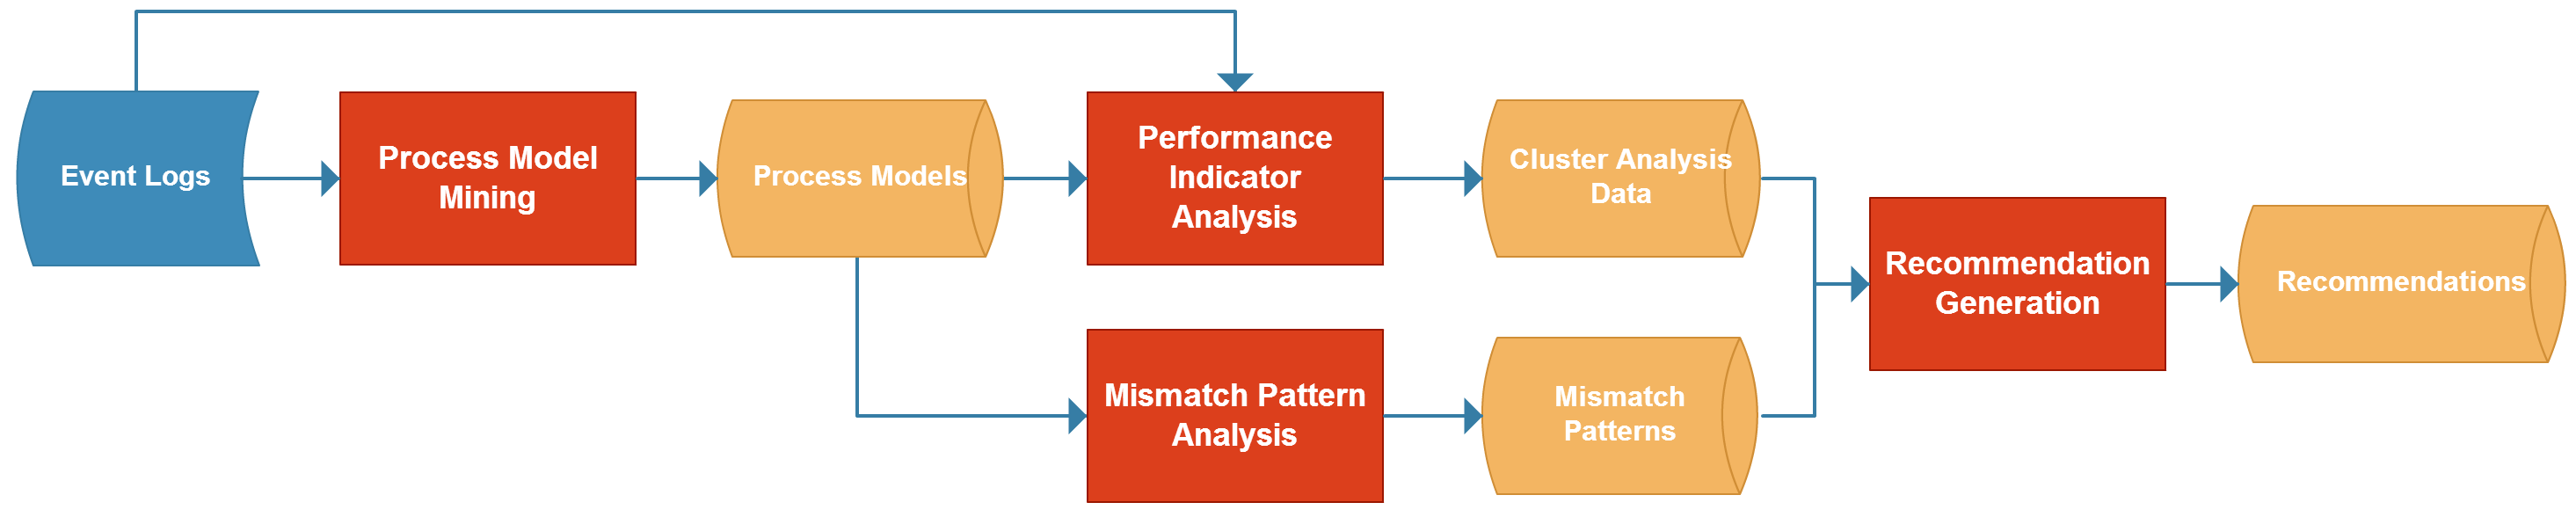
\includegraphics[width=\textwidth]{4_methodology/approach-overview}
  \caption{Overview of Methodology}
  \label{fig:approach-overview}
\end{figure}

\subsection{Process Model Mining}
\label{subsec:process-model-mining}
Process model mining in the proposed approach has the aim of creating reproducible and generalized process models from event logs. Considering the fact that the process models may not be defined beforehand or outdated to reflect latest state of the process, they are mined from event logs. However, if there are process models that represent the event logs, this stage can be skipped. In order to mine process models, implementation of the \textit{Inductive Miner Infrequent (IMi)}, which is proposed in \cite{leemans2014discoveringinfrequent} as an extension to \textit{Inductive Miner} to handle noise in the event logs, is used in this study. In order to set a filtering threshold, a user-provided value between 0 to 1 is added as input to the method in addition to event logs.

\subsection{Performance Indicator Analysis}
\label{subsec:performance-indicator-analysis}
Performance indicator analysis stage focuses on calculating and analyzing the performance values using the event logs and mined process models. This stage consists of mainly two steps as 
\begin{inparaenum}[\itshape a\upshape)]
\item alignment and calculation of performance indicators; and
\item clustering of organizations based on their performance values.
\end{inparaenum}
In order to evaluate the performance of an organization based on their process models and past activities; there is a number of indicators in time dimension, cost dimension and utilization \cite{van2011process}. However, in this study, process related performance values are considered since differences in the process models are studied in the next stages. To this aim, the following performance indicators are calculated and analyzed in this stage of methodology:
\begin{description}
	\item[Average Time Between Activities] For each activity in the process model, average time to reach the next activity is calculated. This is a simple but powerful performance metric for organizations since it can yield the average time to complete one task based on a starting point. From the performance perspective, organizations want to minimize average time between activities to increase their throughput \cite{van2012replaying}. This notion can be defined as follows:
  \theoremstyle{definition}
  \begin{definition}{}
  Average time between activity $A$ and $B$ in organization $i$ is $AvgTime_{A\rightarrow B}^{i} = \frac{\sum_{Case\ c \in Event Log_{i}} TimeBetween_{c}(A,B)}{|Occurences_{Event\ Log_{i}}(A,B)|}$ where
    \begin{enumerate}
      \item $TimeBetween_{c}(A, B) = EndTime_{c}(B) - StartTime_{c}(A)$
      \item $StartTime_{c}(A)$ is start time of activity $A$ in case $c$,
      \item $EndTime_{c}(B)$ is end time of activity $B$ in case $c$,
      \item $|Occurences_{Event Log_{i}}(A, B)|$ is number of occurrences of activity $A$ followed by $B$ in  $Event\ Log_{i}$.
    \end{enumerate}
  \end{definition}
	\item[Standard Deviation of Time Between Activities] Time between activities in real life is not stable and they deviate due to various reasons such as the user responsible of tasks, size and the content of tasks or seasonality \cite{van2011process}. On the other hand, organizations want to be confident about their processes and therefore they want to minimize the deviation in the time between activities. Minimized deviation in time helps organizations to plan, act and re-organize the activities in the processes with high accuracy \cite{van2012replaying}. With the same approach above, the following formulation can be defined:
  \theoremstyle{definition}
  \begin{definition}{}
  Standard deviation time between activity $A$ and $B$ in organization $i$ is $StdDevTime_{A\rightarrow B}^{i} = \sqrt{\frac{\sum_{Case\ c \in Event Log_{i}} [TimeBetween_{c}(A, B) - AvgTime_{A\rightarrow B}^{i}]^{2}}{Occurences_{Event\ Log_{i}}(A,B)} }$ 
  \end{definition}
\end{description}

\subsubsection{Replay and Performance Indicator Calculation}
\label{subsubsec:replay-and-performance-summary}
Replay of event logs on process models is based on the idea of \textit{alignment} which is formalized in \cite{van2012replaying} and the basic assumption in this concept is that process models and event logs have the same activity labels. For each organization, the steps of alignment and creating transitions are performed with the corresponding event logs and process models; and the resulting process performance summaries are used for further analysis. Resulting data can be defined as follows:
  \theoremstyle{definition}
  \begin{definition}{} Performance Summary data for any organization $i$ is $PerfSum_{i}= \{AvgTimeSum_{i}\ \cup\ StdDevTimeSum_{i}\}$ where
    \begin{enumerate}
      \item $AvgTimeSum_{i} = \{ AvgTime_{A \rightarrow B}^{i} | A , B  \in Event\ Log_{i}\}$
      \item $StdDevTimeSum_{i} = \{ StdDevTime_{ A\rightarrow B}^{i} | A, B  \in Event\ Log_{i}\}$
    \end{enumerate}
  \end{definition}

\subsubsection{Performance Indicator Clustering}
\label{subsubsec:performance-indicator-clustering}
Clustering is based on the idea of collecting the set of observations into clusters so that observations within the same cluster are similar whereas the observations from different clusters are dissimilar. In this study, clustering is used to gather organizations based on their performance indicator data. In this research, random initialization based \textit{k-means++} approach from the study of Arthur and Vassilvitskii \cite{arthur2007} is used to cluster organizations. Since the number of clusters are not known priori, k-means clustering is applied starting \textit{k} from 1 to the number of organizations. For each clustering with different number of clusters, \textit{Sum of Squared Error (SSE)} values are plotted and user is asked to select the appropriate cluster size. For the selected cluster size, clustering related information is used to generate recommendations in the further steps. Resulting cluster analysis data is formulated as follows:
\theoremstyle{definition}
\begin{definition}
Cluster Analysis Data is a tuple $(k, Assignments, Cluster\ Centroids)$ where
\begin{enumerate}
  \item $k$ is the number of clusters,
  \item $Assignments$ is a set of tuple $(Organization_{i}, Cluster_{j})$ where $i$ is identifier for organization and $j \leq k$ is identifier for cluster,
  \item $Cluster\ Centroids$ is a set of tuple $(Cluster_{j}, Type, A_{start}, A_{end}, Value)$ where
    \begin{enumerate}
      \item $Type$ is performance indicator type which is $Average$ or $StandardDev$,
      \item $A_{start}$ and $A_{end}$ are starting and ending points of performance indicator,
      \item $Value$ is the actual value of performance indicator,
      \item $Cluster\ Centroids_{j}$ is a function that returns a set of $Centroid$ which is a tuple $(Type, A_{start}, A_{end}, Value)$ for $Cluster_{j}$.
    \end{enumerate} 
\end{enumerate}
\end{definition}

This stage of methodology can be visualized as an input-output system in Figure~\ref{fig:performance-indicator-clustering-blackbox}. 
\begin{figure}
  \centering
  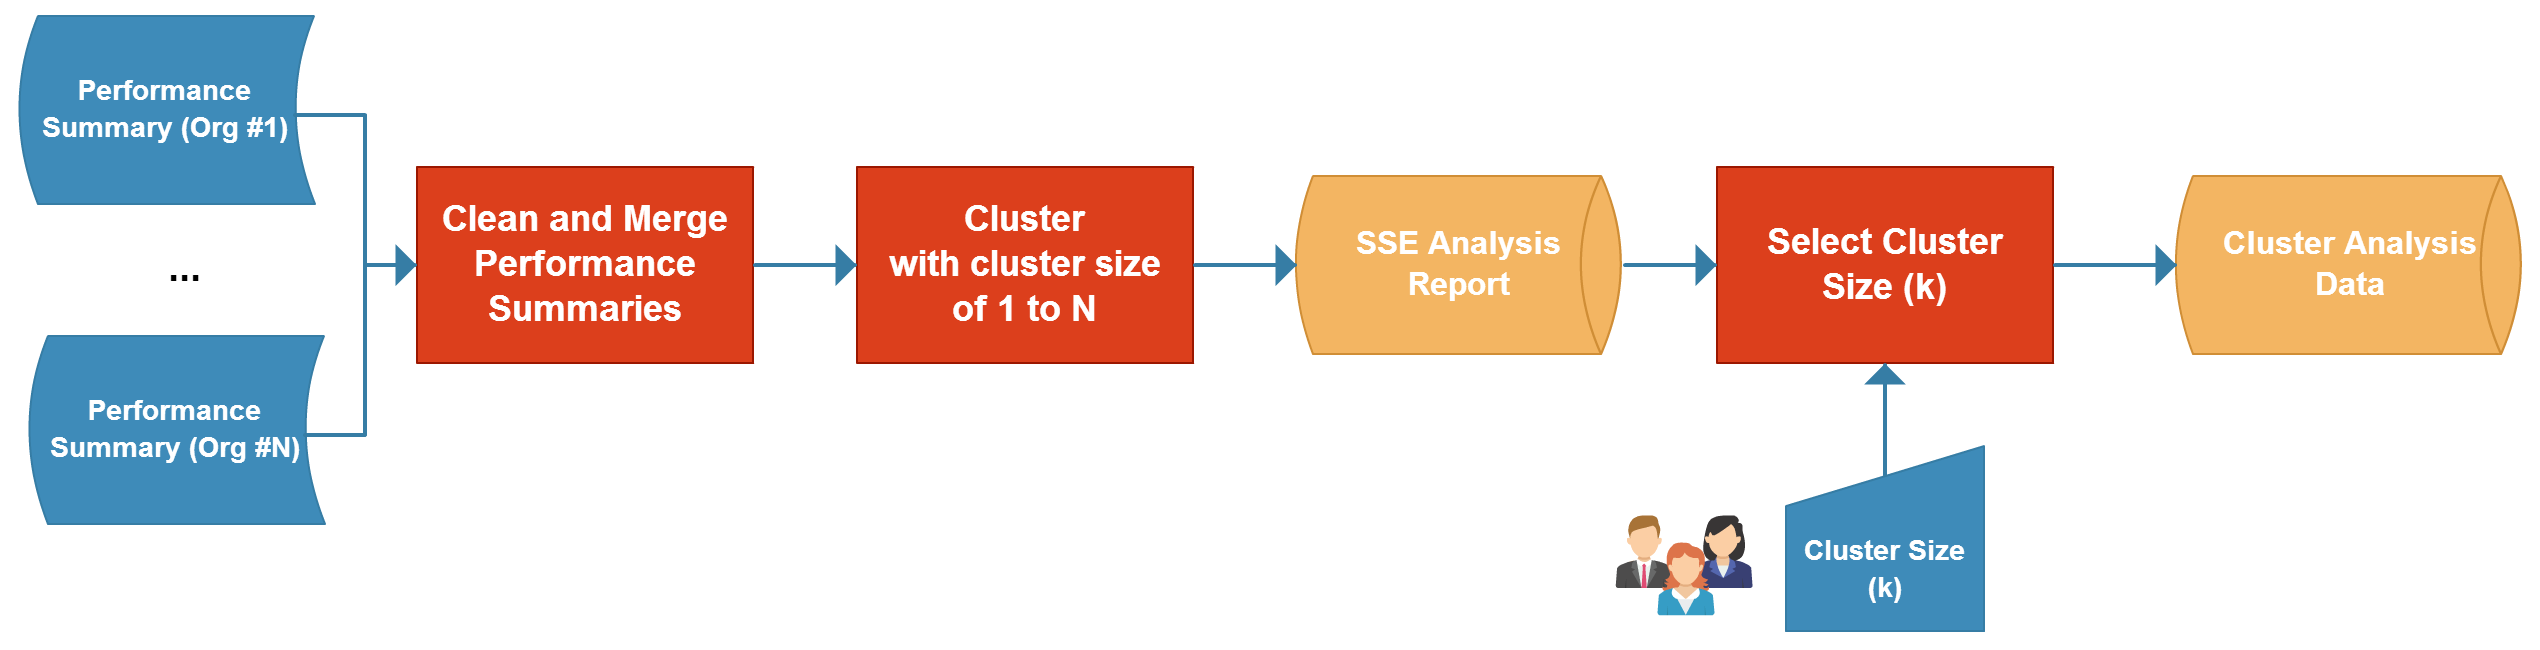
\includegraphics[width=\textwidth]{4_methodology/performance-indicator-clustering-blackbox}
  \caption{Performance Indicator Clustering Stage as Black-box }
  \label{fig:performance-indicator-clustering-blackbox}
\end{figure}

\subsection{Mismatch Pattern Analysis}
\label{subsec:mismatch-pattern-analysis}
In order to learn from other organizations, it is necessary to spot the differences between process models of different organizations. In this phase, differences between process models will be revealed by the mismatch patterns which are defined by Dijkman \cite{dijkman2007mismatch}. Since performance indicators are calculated based on a starting and ending point in the process model, the same approach is applied to locate mismatch patterns. In other words, differences of process models are located through a starting activity to an ending activity. With this aim, each mismatch pattern and its analyzers are defined by extending the following definitions:
\theoremstyle{definition}
    \begin{definition}
    Mismatch Pattern is a tuple ${Mismatch\ Patten} = (O_{1}, O_{2}, ExtensionData, A_{start}, A_{end}) $ where 
    \begin{enumerate}
      \item $O_{1}$ is the first organization and \item $O_{2}$ is the second organization in between the pattern occurs,
      \item $ExtensionData$ is a set of tuples where mismatch related information is recorded, 
      \item $A_{start}$ and $A_{end}$ are starting and ending points to check mismatch patterns.
    \end{enumerate}
    \end{definition}
\theoremstyle{definition}

\begin{definition}
    Mismatch Pattern Analyzer is a function $MismatchPatternAnalyzer(O_{1}, O_{2}, A_{start}, A_{end})$ and it returns a set of \textit{Mismatch Pattern} for the organization $O_{1}$ compared to $O_{2}$ for the activities between $A_{start}$ and $A_{end}$.
\end{definition}

For each organization, mismatch patterns are gathered and stored for the further analysis as visualized in Figure~\ref{fig:mismatch-pattern-analysis-blackbox}.
\begin{figure}
  \centering
  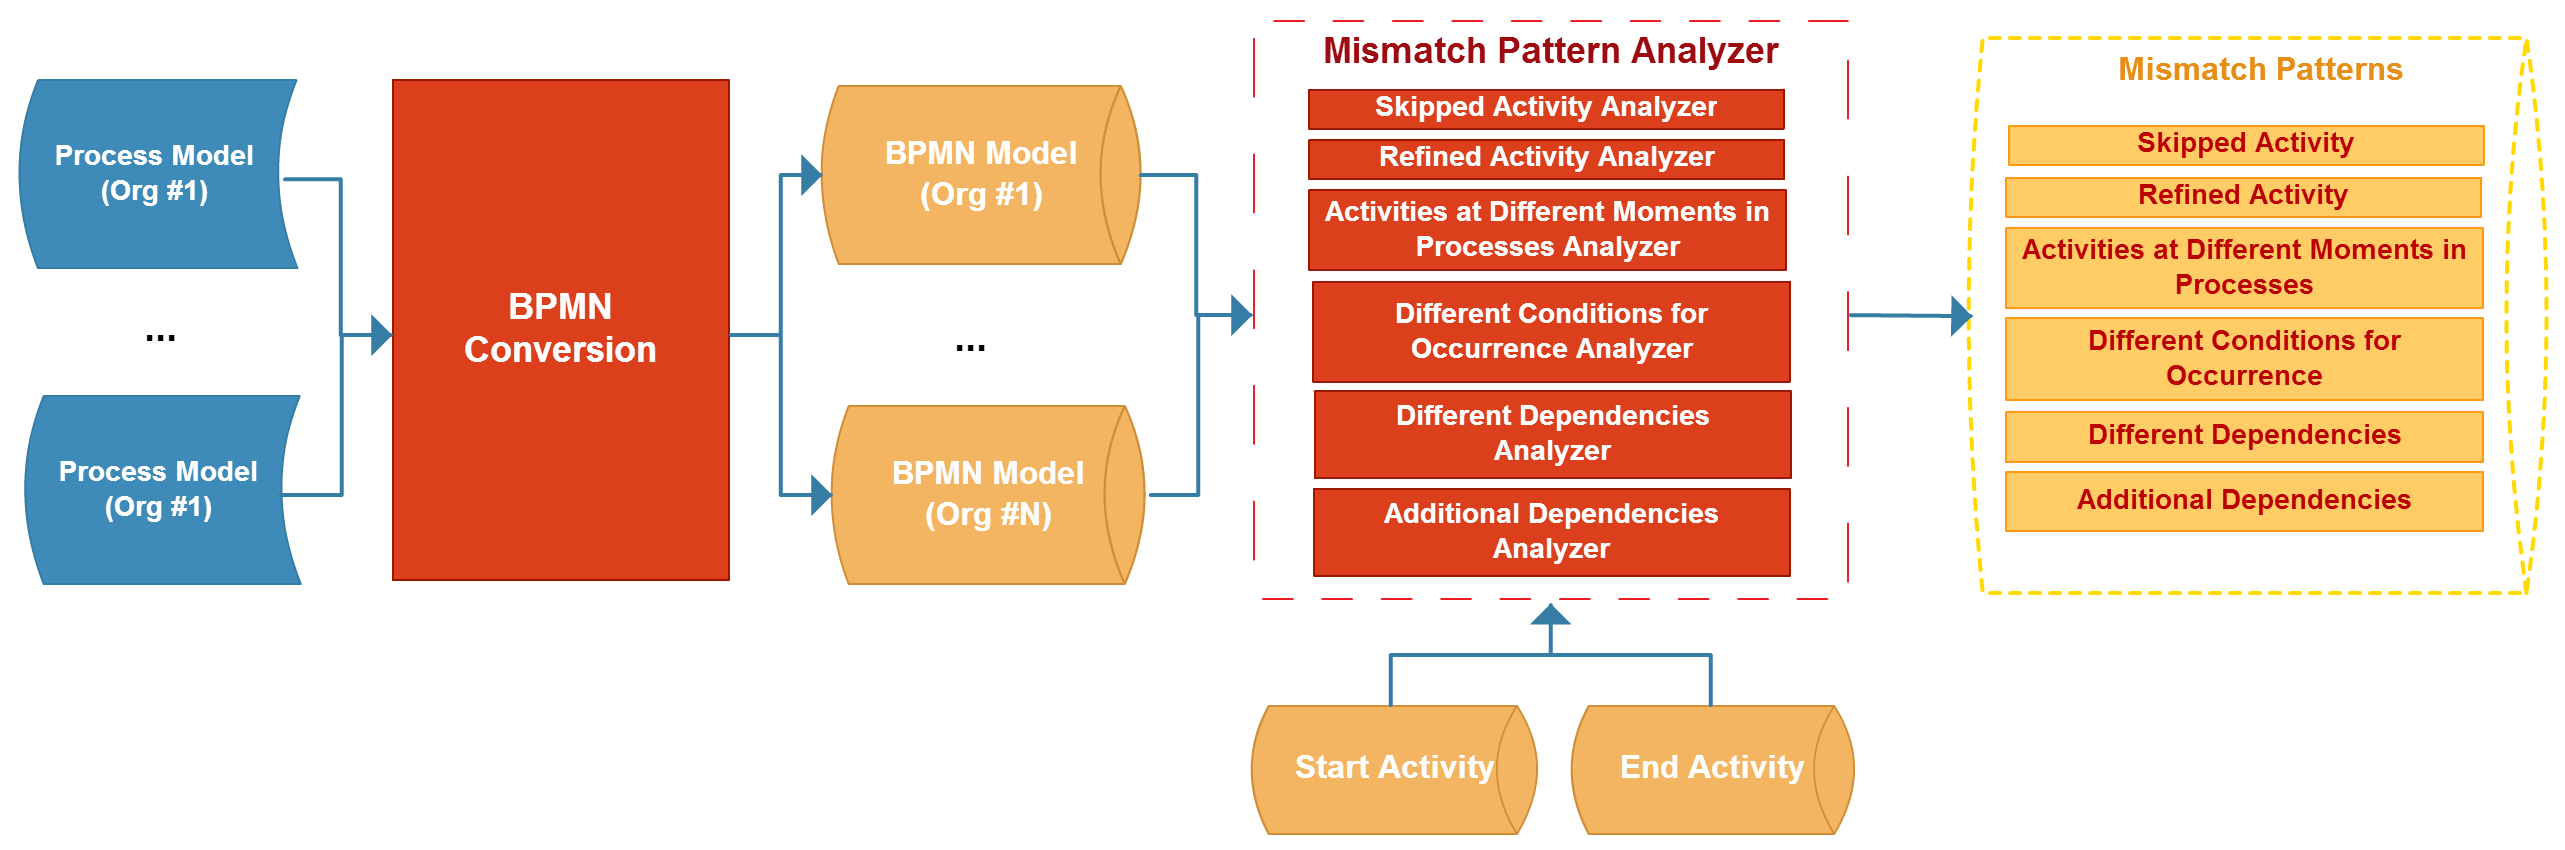
\includegraphics[width=\textwidth]{4_methodology/mismatch-pattern-analysis-blackbox}
  \caption{Mismatch Pattern Analysis Stage as Black-box}
  \label{fig:mismatch-pattern-analysis-blackbox}
\end{figure}

\subsection{Genarating Suggestions/Recommendations for Performance Improvement}
\label{subsec:recommendation-generation}
\theoremstyle{definition}
Recommendation generation stage in the methodology is the final and core stage where all information retrieved from the event logs until now are utilized. In this study, idea of recommendation is based on providing a set of mismatch patterns for each organization so that they can enhance their processes. These mismatch patterns are generated by comparing the process models of other organizations, particularly those that are performing better in terms of their performance indicator values. Recommendation idea and recommendation generation function is defined as following:
\begin{definition}
Recommendation is a tuple ${Recommendation} = (O, A_{start}, A_{end}, Mismatch\ Patterns) $ where 
  \begin{enumerate}
    \item $O$ is identifier for organization,
    \item $A_{start}$ and $A_{end}$ are starting and ending activities in between the recommendations are checked,
    \item $Mismatch\ Patterns$ is collection of mismatch patterns.
  \end{enumerate}
\end{definition}

\theoremstyle{definition}
\begin{definition}
Recommendation generation is a function that is $RecGen(O, C, P)$ and it returns a set of $Recommendation$ where
  \begin{enumerate}
    \item $O$ is identifier for organization,
    \item $C$ is \textit{Cluster Analysis Data} which is result of cluster analysis stage,
    \item $P$ is \textit{Performance Threshold} which is a real number larger than or equal to 0 and it is calculated over the same type of performance indicators of different organizations in \textit{Cluster Analysis Data}.
  \end{enumerate}
\end{definition}

Algorithm of recommendation generation function is based on the idea of checking other clusters for a significant change in performance indicators, where significance is defined by the threshold provided by user. After finding significant difference, all organizations in other clusters are checked against mismatch patterns with the starting and ending activities defined in performance indicators. Only mismatches which are located between the activities that causes high level of difference in performance indicators are analyzed. This approach is formalized in Algorithm~\ref{algo:recgen}.
 \begin{algorithm}
\DontPrintSemicolon % Some LaTeX compilers require you to use \dontprintsemicolon instead 
\KwIn{$O$ organization, $C$ Cluster Analysis Data, $P$ performance difference threshold}
\KwOut{$Recommendations$ a set of recommendations}
$Recommendations \leftarrow \{\}$ \;
$i \leftarrow C(Assignments(O))$ \;
\For{$Centroid \in C(Cluster Centroids_{i})$} { 
  \For{$Centroid' \in C(Cluster Centroids_{j})\ i\neq j$} { 
    \If{$Centroid(A_{start}) = Centroid'(A_{start})\ \&\ Centroid(A_{end}) = Centroid'(A_{end})$} {
      \If{ ($\left |  Centroid(Value) -  Centroid'(Value)\right | \div Centroid(Value)) \geq P$  } {
        $A_{start} \leftarrow Centroid(A_{start})$ \;
        $A_{end} \leftarrow Centroid(A_{end})$ \;
        $MismatchPatterns \leftarrow \{\}$ \;
        \For{$O' \in C(Assignments(j))$} {
          $MismatchPatterns$ \leftarrow  Mismatch Pattern Analysis($O$,$O'$,$A_{start}$,$A_{end}$) \;
        }
        $Recommendations$ \leftarrow  Recommendation($O$,$A_{start}$,$A_{end}$, $MismatchPatterns$) \;
      }
    }
  }
}
\Return{$Recommendations$} \;
\caption{Recommendation Generation}
\label{algo:recgen}
\end{algorithm}
This stage of methodology can be visualized as gathering inputs of mismatch patterns data and cluster analysis data in Figure~\ref{fig:recommendation-generation-blackox}.
\begin{figure}
  \centering
  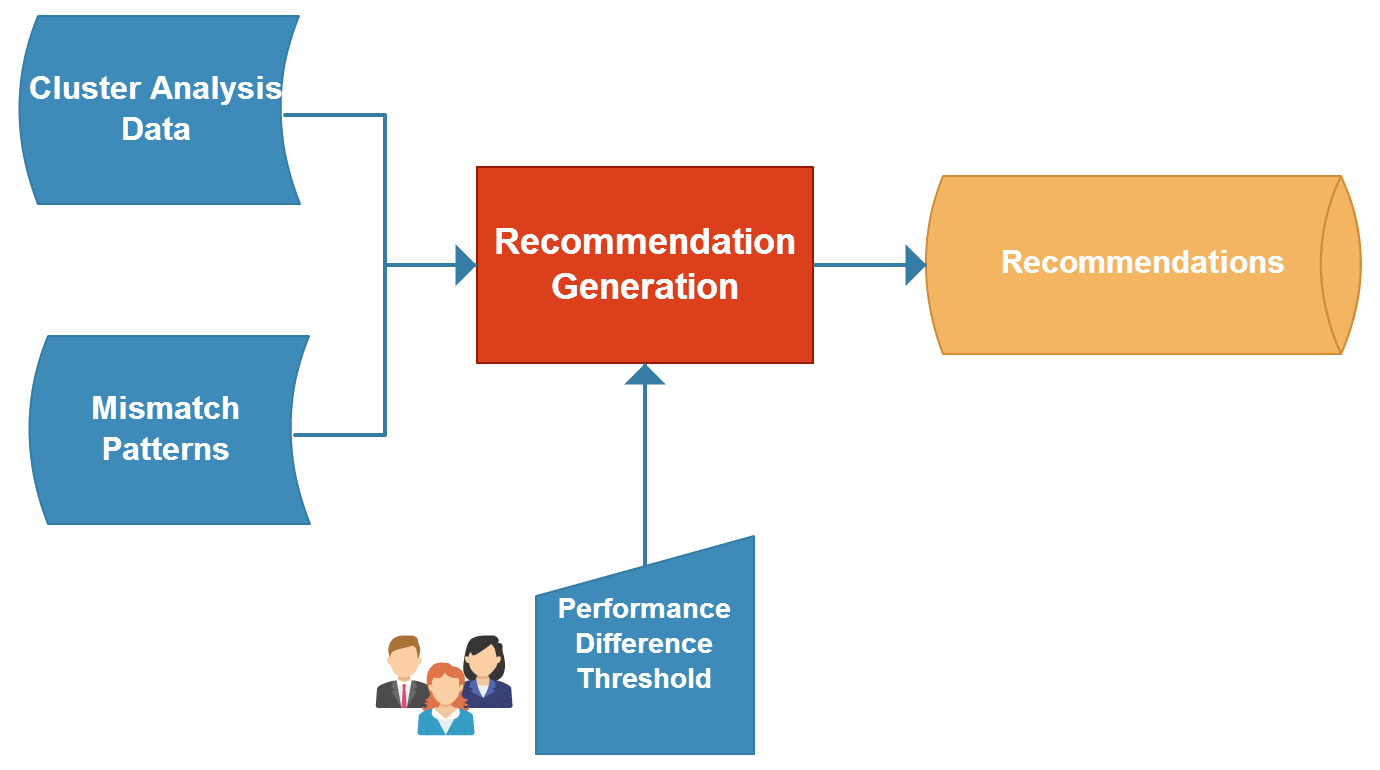
\includegraphics[width=0.5\textwidth]{4_methodology/recommendation-generation-blackbox}
  \caption{Recommendation Generation Stage as Black-box}
  \label{fig:recommendation-generation-blackox}
\end{figure}

\subsection{Implementation in ProM Framework}
\label{subsec:implementation}
Methodology of this study is implemented in ProM \cite{verbeek2010prom}, which is an extensible framework that supports a wide variety of process mining techniques in form of plugins. Approach of this study is implemented with its each stage as a standalone plugin that enables extensions for further studies. Developed set of plugins are packaged with the name of \textit{CrossOrgProcMin}\footnote{\url{http://www.promtools.org/prom6/packages/CrossOrgProcMin}} and published open-source\footnote{\url{http://github.com/onuryilmaz/cross-org-proc-min}} being available in the latest version of ProM release.

\bibliographystyle{splncs03}
\bibliography{7_references/references}


\end{document}
